\section{Method}
\label{sec:meth}

% - spatial signatures
% -- SS as a characterisation of space based on F and F - very brief intro
% -- components can be studies independently
%   -- this paper focuses on form component only
Urban morphology tends to consider form only when trying to understand urban
environment, leaving aside its functional aspects from population and amenities to green
and blue spaces. However, one can argue that only combination of form and function can
provide deeper insights into the complexity of cities. The notion of \textit{spatial
signatures} combines both aspects into a single model, defined as:

\newtheorem*{theorem}{}
\begin{theorem}
    A characterisation of space based on form and function designed to understand urban
environments
\end{theorem}

Spatial signatures then provide a typology of space defined by both form and function
together, encoding the interplay between the two. On the other hand, not all questions
can be answered using both components at the same time. Each of them, form as well as
function, can be studied independently when needed. This paper explores the form component
of spatial signatures characterisation and derives form-based signatures as a
single-aspect classification of space.

% - spatial unit -- spatial unit criteria -- issues with available units -- proposal of
%   enclosed tessellation -- brief description and a reference to conceptual?
Spatial signatures are conceptually defined as an aggregation of granular elements into
contiguous areas based on the homogeneity of their characterisation. That poses a first
methodological question - which spatial unit should be used for capturing of such
characterisation? The optimal unit should be \textit{indivisible} - when split into
smaller components, none of them would be enough to encode character of a signature;
\textit{internally consistent} - each observation should reflect single signature type;
and geographically \textit{exhaustive} - every location in the area of interest, both
built-up and un-built, should be covered.

Literature tends to be split into three groups when it comes to unit of analysis. One
uses predefined administrative boundaries (REF) but that can be seen as a suboptimal
solution as their definition follows different goals and some even argue that
“administrative units obscure morphologic reality” \citep{taubenbock2019new}. The other
employs uniform grids, in some cases linked to a spatial index (like hexagonal H3 grid
\citep{brodsky2018h3}) or to other types of data commonly distributed on grids (e.g.
\cite{jochem2020}). However, grids cells are rarely indivisible and often internally
inconsistent as their definition does not reflect the spatial configuration on the
ground. The most common approach in urban morphology is to use structural elements as
buildings \citep{hamaina2012a}, street segments \citep{araldi2019} or plots
\citep{berghauserpont2019a} as a unit. However, these are not exhaustive as they are not
present in un-built areas. Plots would theoretically provide geographical exhaustiveness
but since their conceptual definition is not stable and geometric representation varies
\citep{kropf2018plots}, they are unfit for a large scale analysis.

We propose to use an alternative spatial unit named \textit{enclosed tessellation cell}
(EC), defined as:

\begin{theorem}
    The portion of space that results from growing a morphological tesselation within an
enclosure delineated by a series of natural or built barriers identified from the
literature on urban form, function and perception.
\end{theorem}

\martin{We should somehow cite the conceputal paper when we talk about signatures and EC}

The ECs are generated in three steps illustrated on a figure \ref{fig:et_diagram}.
First, a defined set of spatial features that divide space into smaller parts
(\ref{fig:et_diagram}A) is integrated into a single set of boundaries
(\ref{fig:et_diagram}B). Such boundaries are usually formed by linear features as street
network, railway or rivers. Second, these boundaries are used to subdivide space into
\textit{enclosures}, a smaller areas delimited from all sides by at least one boundary
feature (\ref{fig:et_diagram}C). Third, enclosures are combined with building footprints
taking the role of anchors in space and subdivided into ECs based on proximity to each
building, using a morphological tesselation algorithm
\citep{fleischmann2020morphological} (\ref{fig:et_diagram}D).

\begin{figure}
    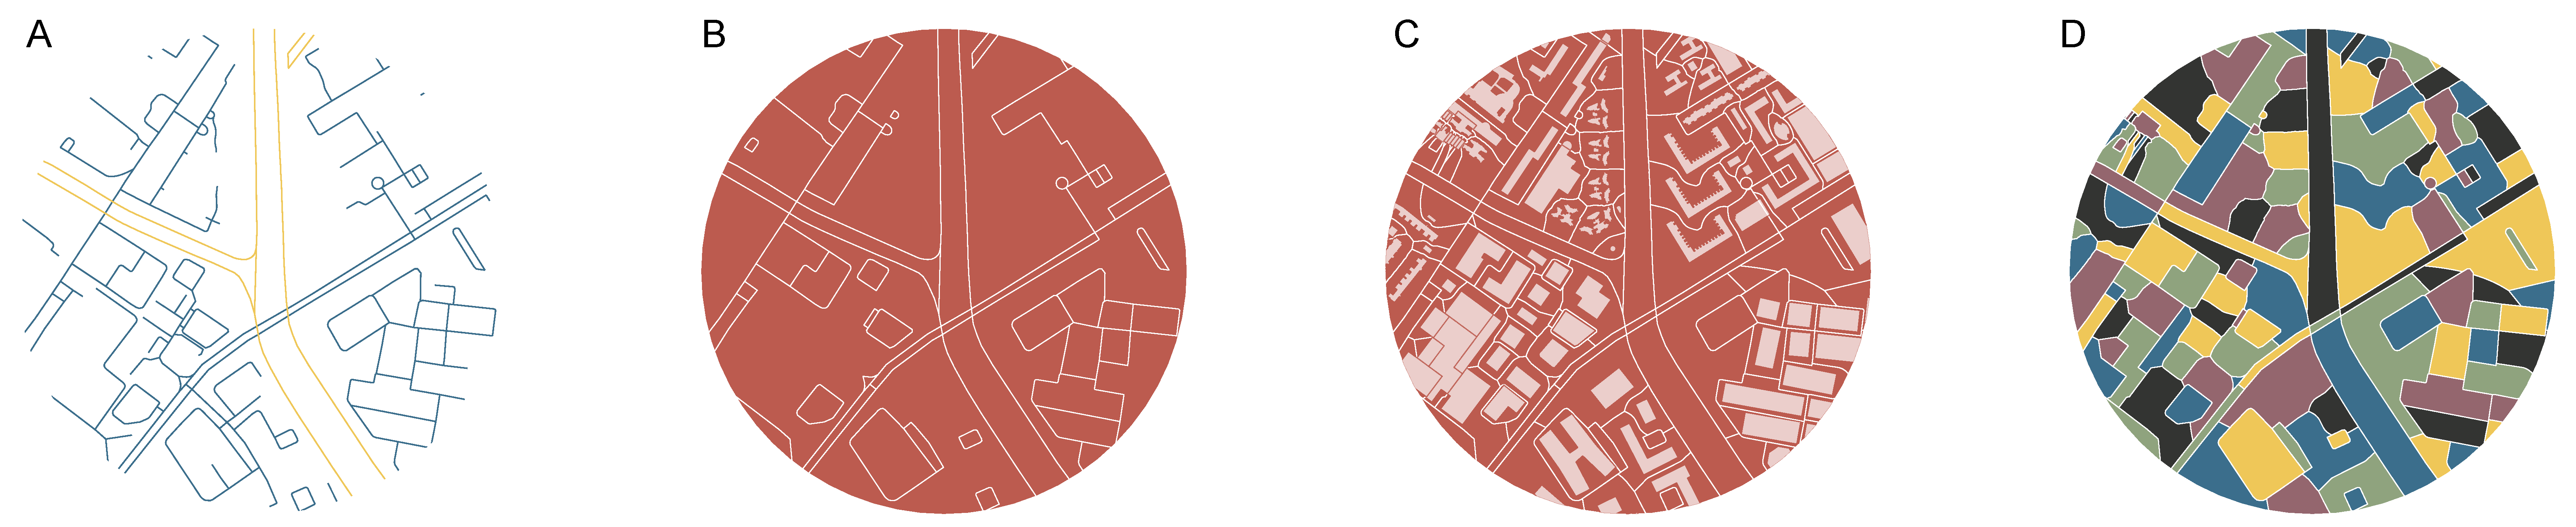
\includegraphics[width=\linewidth]{figures/et_diagram.pdf}
    \caption{Diagram illustrating the sequential steps leading to the delineation of
    enclosed tessellation. From a series of enclosing components, where blue are streets
    and yellow river banks (A), to enclosures (B), incorporation of buildings as anchors
    (C) to final tessellation cells (D).}
    \label{fig:et_diagram}
\end{figure}

Resulting ECs are indivisible and internally consistent, as they are very granular and
linked at maximum to a single building, and exhaustive as they cover entirety of space
thanks to contiguous geometry of enclosures. Their structure and scale adapts to the
environment and can take a form of a small-scale granular mesh in city centres of
historical origin as well as large-scale polygons encoding the vast natural open spaces.

% - morphometrics
% -- characterisation of building patterns using morphometrics
% -- the principle of inclusiveness (more better) to minimise selection bias
% - context
% -- representation of context as topological distance
% -- reflection of distribution of characters
Having ECs, building footprints and street networks, we measure a wide range of aspects
of their spatial organisation, from dimensions and shapes of individual objects to their
spatial distribution, intensity or connectivity reflecting configuration of streets. We
call these measurements \textit{morphometric characters}. Since we do not a-priori know
which characters are determining the differences between types of urban
development the most, we aim to include a relatively large set of characters to
avoid potential selection bias, believing that further steps will be able to deal with a
larger amount of input data generated by a larger number of characters\footnote{The list
of measured morphometric characters and their implementation details are available in
the online repository at github.com/urbangrammarai/spatial\_signatures.}. As the aim is
to use these characters to detect contiguous homogenous areas of urban form, we are more
interested in tendencies of their distributions within space. Therefore, we link all
values to ECs and capture the distribution of each within a spatial context
around each EC. Context here is defined as a topological distance (10 steps) on enclosed
tessellation and each EC in reach is weighted by its distance to the original EC. This
kind of aggregation is adaptive to the pattern of ECs and reflects the higher importance
of close elements compared to more distant ones.

% - clustering & dissolution
% -- K-Means clustering of ET cells based on morphometric profile
% -- hierarchical approach - sub-dividing interesting clusters via second level K-Means
% -- aggregation of cells into form-based signatures
ECs characterised by contextualised morphometric characters are clustered using K-Means
clustering algorithm, deriving a typology of ECs. Even though K-Means itself does not
contain any contiguity constraint, the design of inherently spatially autocorrelated
characters results in clusters that are spatially contiguous anyway. Moreover, the clustering can
be potentially applied hierarchically. When further detail is needed, individual
clusters can be clustered again resulting in a hierarchy of classes. Finally, ECs are
aggregated together based on their class, creating geometry of spatial signatures, where
each contiguous area classified as a single cluster represents a single signature.

% - case study - GB
We test the method on the case study covering the whole Great Britain, illustrating both
potential and limits of the analysis of urban form at scale.

% - data
% -- input data in general
% -- input data in the GB
% -- OS Open Map
% --- potential limitation of open data
% -- OS Open Roads
The method itself requires a relatively available data on input. First, a set of
barriers encoding delimiters of enclosures is needed. In our case, we use street
networks from OS OpenRoads (REF), representing street centrelines, railways from OS
OpenMap Local (REF), rivers from OS OpenRivers and a coastline from OS Strategi® (REF),
all released as open data under a permissive license allowing us to release
resulting classification as an open data product. Second input is the layer capturing
building footprints, which is again retrieved from the OS OpenMap Local. However, the
data reflect aggregated footprints and do not distinguish between individual buildings
when they are adjacent. While that is indeed a limitation, the method is designed and
tested (REF Conceptual paper??) to be robust enough to accommodate for various
sub-optimal data sources.
